\documentclass{standalone}
\usepackage{fontspec}
\setsansfont{DejaVuSans.ttf}[Path=./,Kerning=Off,Ligatures={TeXOff,NoCommon}]
\usepackage{tikz}
\begin{document}
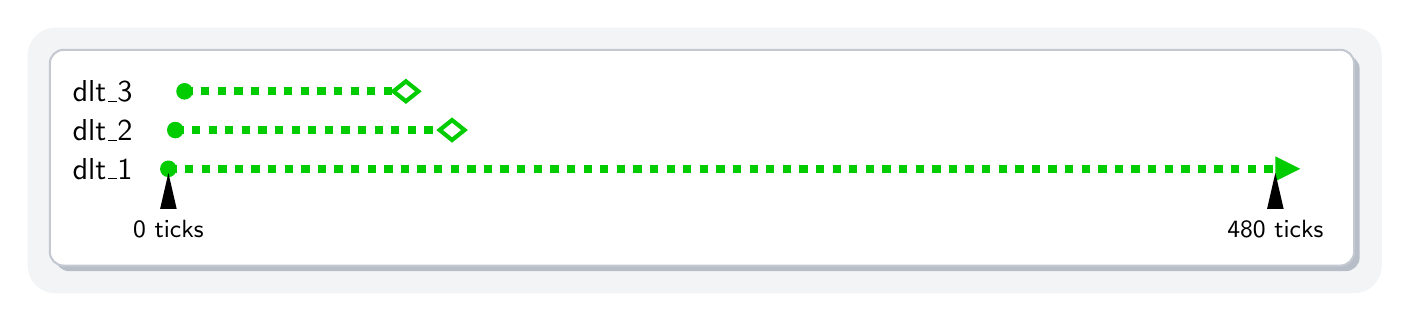
\begin{tikzpicture}[x=1pt,y=1pt,miter limit=4,font=\sffamily]
\definecolor{ts000000}{HTML}{000000}
\definecolor{ts00CC00}{HTML}{00CC00}
\definecolor{tsB8BEC8}{HTML}{B8BEC8}
\definecolor{tsC4C9D1}{HTML}{C4C9D1}
\definecolor{tsF3F4F6}{HTML}{F3F4F6}
\definecolor{tsFFFFFF}{HTML}{FFFFFF}
\begin{scope}[shift={(16,16)}]
\path[rounded corners=10pt,fill=tsF3F4F6] (0,0) rectangle (489.3088,95.9766);
\path[rounded corners=5pt,fill=tsB8BEC8] (10,8) rectangle (481.3088,85.9766);
\path[rounded corners=5pt,fill=tsFFFFFF,draw=tsC4C9D1,line width=0.75pt] (8,10) rectangle (479.3088,87.9766);
\path[draw=ts00CC00,line width=3pt,dash pattern=on 3pt off 3pt] (50.8501,44.9766) -- (450.8501,44.9766);
\path[fill=ts00CC00] (50.8501,44.9766) circle[radius=3];
\path[fill=ts00CC00] (459.8501,44.9766) -- (450.8501,49.4766) -- (450.8501,40.4766) -- cycle;
\path[draw=ts00CC00,line width=3pt,dash pattern=on 3pt off 3pt] (53.3501,58.9766) -- (148.8501,58.9766);
\path[fill=ts00CC00] (53.3501,58.9766) circle[radius=3];
\path[draw=ts00CC00,line width=1.5pt] (148.8501,58.9766) -- (153.3501,62.5766) -- (157.8501,58.9766) -- (153.3501,55.3766) -- cycle;
\path[draw=ts00CC00,line width=3pt,dash pattern=on 3pt off 3pt] (56.6834,72.9766) -- (132.1834,72.9766);
\path[fill=ts00CC00] (56.6834,72.9766) circle[radius=3];
\path[draw=ts00CC00,line width=1.5pt] (132.1834,72.9766) -- (136.6834,76.5766) -- (141.1834,72.9766) -- (136.6834,69.3766) -- cycle;
\path[fill=ts000000] (50.8501,43.4766) -- (47.8501,30.4766) -- (53.8501,30.4766) -- cycle;
\path[fill=ts000000] (450.8501,43.4766) -- (447.8501,30.4766) -- (453.8501,30.4766) -- cycle;
\node[anchor=base west,inner sep=0,font=\sffamily\fontsize{11}{12.8047}\selectfont,text=ts000000] at (16,69.1685) {dlt\_3};
\node[anchor=base west,inner sep=0,font=\sffamily\fontsize{11}{12.8047}\selectfont,text=ts000000] at (16,55.1685) {dlt\_2};
\node[anchor=base west,inner sep=0,font=\sffamily\fontsize{11}{12.8047}\selectfont,text=ts000000] at (16,41.1685) {dlt\_1};
\node[anchor=base,inner sep=0,font=\sffamily\fontsize{9}{10.4766}\selectfont,text=ts000000] at (50.8501,20.1226) {0 ticks};
\node[anchor=base,inner sep=0,font=\sffamily\fontsize{9}{10.4766}\selectfont,text=ts000000] at (450.8501,20.1226) {480 ticks};
\end{scope}
\end{tikzpicture}
\end{document}
